Uncertainties on the unfolded result are evaluated using error propagation, consistent with the standard approach used at ATLAS.
Uncertainties are split into sources (sometimes called ``uncertainty components'') that are each treated as uncorrelated to each other.
For each such uncertainty source, a perturbation is introduced either to the MC or data corresponding to its impact: $+1\sigma$, and in case of two-sided uncertainties, also $-1\,\sigma$. For each uncertainty perturbation $u$, the unfolding (``full analysis'') is then repeated using the modified samples, which results in a OmniFold weight $\nu_{u}(\vec{x})$ that is slightly different from the nominal OmniFold weight $\nu(\vec{x})$. 
Each event $i$ in the unfolded dataset is hence assigned one nominal weight $w_{i}$ and a list of alternative weights $w_{iu}$, where the index $u$ corresponds either to a systematic uncertainty source, or statistical replica variation. 

The uncertainty amplitude $\Delta_{ku}$ of any bin $k$ associated with uncertainty source $u$ is now evaluated as the different between the perturbed and nominal result:
\begin{equation}
  \Delta_{ku} = \hat{\sigma}_{ku} - \hat{\sigma_k},
\end{equation}
where both $\hat{\sigma}_k$ terms are evaluated according to equation~\ref{eq:fid-xsec}.

% These weights can be normalized according to:
% \begin{equation}
%   \label{eq:xsec-norm}
%   w_{i} = \frac{\nu_{i}\,w^\mathrm{nom}_{i}}{\mathcal{L}},
% \end{equation}
% where $w^\mathrm{nom}_{i}$ is the nominal MC weight that includes the normalization according to $\sigma\,\mathcal{L}$ (i.e.\ used in figures~\ref{fig:MuActual}-\ref{fig:trackInfo}), $\nu_{i}$ is the OmniFold (or MultiFold) weight that corrects (unfolds) the MC prediction to data, and $\mathcal{L}$ is the integrated luminosity of the dataset. The weights $w_i$ defined according to Eq.~\ref{eq:xsec-norm} now has units of cross section and the sum of such weights of all events that fall in any fiduciary region will constitute a measurement of the associated fiducial cross section. This can be written as:
% \begin{equation}
%   \label{eq:fid-xsec}
%   \hat{\sigma}_{k} = \sum_{i}^{N_\mathrm{events}}w_{i}\,\mathcal{I}[b(\vec{x}_{i})=k],
% \end{equation}
% where $b(\vec{x}_{i})$ returns an index $k\in\{0,1,2,...,n_\text{bins}\}$ corresponding to the fiducial region event $i$ falls in (based on its features $\vec{x}_i$), 
% and $\mathcal{I}[\cdot]$ is the indicator function that is 1 when $\cdot$ is true and zero otherwise.


\subsection{Data and Monte Carlo statistical uncertainties}
Statistical uncertainties will be evaluated using bootstrapping~\cite{ATLAS-bootstrap}.  A set of $N_\mathrm{BS}$ pseudo-datasets are constructed where each event $i$ has a weight $W_{ib}\,w^\text{nom}_i$, where $w^\text{nom}_{i}$ is unity for data and assigned according to equations~\ref{eq:mc-norm} or~\ref{eq:mc-norm-reco} for simulation. $W_{ib}$ is a value sampled randomly from a Poisson distribution with a mean of unity, which is done separately for each event $i$ and bootstrap replica $b$.  To ensure that the ``uncertainty on the uncertainty'' is negligible an ensemble of $N_\mathrm{BS} \gtrsim 100$ such pseudo-datasets can be used.
Using these ensembles, uncertainties are straightforward to compute as outlined below, however it is computationally expensive to perform the full analysis on each of the $N_\mathrm{BS}$ bootstrap replicas, and thus we will compute them once all other results are finished.

As described above, for data statistical uncertainties, $N_\mathrm{BS}^\mathrm{ds} \approx 100$ bootstrap replica datasets are produced from actual data events.
The difference between these datasets, which can be seen by plotting any distribution, will reflect the data statistical uncertainty.
The full analysis will be performed for each such datasets with the nominal MC sample, and each event $i$ will hence get $N_\mathrm{BS}$ OmniFold weights $\nu_{ip}$. 
Similarly, the MC statistical uncertainties is evaluated using the nominal data, but with MC events fluctuated $N_\mathrm{BS}^\mathrm{ms}$ times, which will result in $N_\mathrm{BS}^\mathrm{ms}$ different OmniFold weights.

The unfolded cross section $\sigma_{kb}$ for any given bin $k$ can be evaluated for each bootstrap replica $b$ (see equation~\ref{eq:fid-xsec}), and the standard  deviation of such estimates $\Delta_{k}$ constitutes the associated statistical uncertainty:
\begin{eqnarray}
  \label{eq:bs}
  \bar{\sigma}_k = \frac{1}{N_\mathrm{BS}}\sum_{b=1}^{N_\mathrm{BS}} \hat{\sigma}_{kb} 
  & & \text{(bootstrap mean)}\\
  V_k = V[\hat{\sigma}_k] = \Delta_k^2 = \frac{1}{N_\mathrm{BS}}\sum_{b=1}^{N_\mathrm{BS}} \left(\hat{\sigma}_{kb} - \bar{\sigma}_k\right)^2 
  & & \text{(stat. variance)}\\
  C_{kl} = \mathrm{COV}[\hat{\sigma}_k,\hat{\sigma}_l] = \frac{1}{N_\mathrm{BS}}\sum_{b=1}^{N_\mathrm{BS}} \left(\hat{\sigma}_{kb} - \bar{\sigma}_k\right)\,\left(\hat{\sigma}_{lb} - \bar{\sigma}_l\right) 
  & & \text{(stat. covariance)}
\end{eqnarray}

Any bin $k$ will hence have a data statistical uncertainty $\Delta_k^\mathrm{ds}$ and MC statistical uncertainty $\Delta_k^\mathrm{ms}$.
Note also that the statistical correlation between two bins is given by $\rho_{kl} = C_{kl}/(\Delta_k\,\Delta_l).$


% Each event will have $N$ weights associated with the data statistical uncertainty and from this, one can compute the covariance matrix for any particular binning scheme $b(x)\in\{0,1,2,...,n_\text{bins}\}$:

% \begin{align}
% \mathbb{E}_k &= \frac{1}{N}\sum_{j=1}^N\sum_{i=1}^{N_\text{events}} w_{ij} \mathbb{I}[b(x_i)=k]\\
% \mathbb{E}_{kk'} &= \frac{1}{N}\sum_{j=1}^N \left(\sum_{i=1}^{N_\text{events}} w_{ij} \mathbb{I}[b(x_i)=k]\right)\left(\sum_{i=1}^{N_\text{events}} w_{ij} \mathbb{I}[b(x_i)=k']\right)\\
% \Sigma_{kk'}&=\mathbb{E}_{kk'} - \mathbb{E}_k\mathbb{E}_{k'}\,,
% \end{align}
% %
% where $w_{ij}$ is the OmniFold weight for bootstrap $j$ and event $i$, $0\leq k,k'\leq n_\text{bins}$ and $\mathcal{I}[\cdot]$ is the indicator function that is 1 when $\cdot$ is true and zero otherwise.

\subsubsection{Statistical uncertainties on the systematic uncertainties}
\label{sec:uncertaintyuncertainty}

In order to determine if a particular systematic uncertainty is statistically significant and/or to perform uncertainty smoothing, it is necessary to have a statistical uncertainty on the systematic uncertainties. This can be also be achieved using bootstrapping (see section 3.6 of Ref.~\cite{ATLAS-bootstrap}), in fact using the same ensemble of $N_\mathrm{BS}^\mathrm{ms}$ bootstrap replicas as used for the MC statistical uncertainty. The procedure is analogous to the one described in the previous section: evaluate the uncertainty $\Delta_{kub}$ on bin $k$ from source $u$ for each bootstrap replica $b$ and take the standard deviation $\delta_{ku}$ across all bootstrap replicas as the 'uncertainty on the uncertainty'. That is:
\begin{eqnarray}
  \label{eq:unc-on-unc}
  \bar{\Delta}_{ku} = \frac{1}{N_\mathrm{BS}}\sum_{b=1}^{N_\mathrm{BS}} \Delta_{kub} 
  & & \text{(bootstrap uncertainty mean)}\\
  \delta_{ku}^2 = \frac{1}{N_\mathrm{BS}}\sum_{b=1}^{N_\mathrm{BS}} \left(\Delta_{kub} - \bar{\Delta}_{ku}\right)^2 
  & & \text{(stat.~unc.~on systematics)}.
\end{eqnarray}
The uncertainty of bin $k$ for systematic source $u$ is hence given by: $\Delta_{ku} \pm \delta_{ku}$ \todo{or we probably should use the mean variation?: $\bar{\Delta}_{ku} \pm \delta_{ku}$?}.
%The overall uncertainty is given by the MC statistical uncertainty described in the previous section.  However, the experimental uncertainties are highly correlated and so additional boostrapping is required.  In particular, the same bootstrap weights $W_{ib}$ are used for all uncertainty variations and a set of bootstrap weights from the unfolding are produced: $W_\text{pseudo}\times\{w_\text{nominal},w_\text{syst 1}, w_\text{syst 2},...\}$.  In cases where the systematic uncertainty weight is the same as the nominal, then only the features change while the weights are the same.  Then, in a given bin $k$, we can compute 
% \begin{align}
% \mathbb{E}_k^\text{nominal} &= \frac{1}{N}\sum_{j=1}^N\sum_{i=1}^{N_\text{events}} w_{ij,\text{nominal}} \mathbb{I}[b(x_i)=k]\\
% \mathbb{E}_k^\text{$\ell$} &= \frac{1}{N}\sum_{j=1}^N\sum_{i=1}^{N_\text{events}} w_{ij,\text{syst $\ell$}} \mathbb{I}[b(x_i)=k]\\
% \mathbb{E}_{k}^\text{nominal,$\ell$} &= \frac{1}{N}\sum_{j=1}^N \left(\sum_{i=1}^{N_\text{events}} w_{ij,\text{nominal}}\mathbb{I}[b(x_i)=k]\right)\left(\sum_{i=1}^{N_\text{events}} w_{ij,\text{syst $\ell$}}\mathbb{I}[b(x_i)=k]\right)\\
% \Sigma_{k}^\text{nominal,$\ell$}&=\mathbb{E}_{k}^\text{nominal,$\ell$}- \mathbb{E}_k^\text{nominal}\mathbb{E}_k^\text{$\ell$} \,,
% \end{align}
% where $w_{ij,\text{nominal}}$ ($w_{ij,\text{syst $\ell$}}$) is the nominal (systematic uncertainty) OmniFold weight for bootstrap $j$ and event $i$, $0\leq '=k\leq n_\text{bins}$ and $\mathcal{I}[\cdot]$ is the indicator function that is 1 when $\cdot$ is true and zero otherwise.   The statistical uncertainty on the systematic uncertainty is then the square root of $\Sigma_{k}^\text{nominal,$\ell$}$. Note that this requires storing all $N$ weights for each uncertainty\footnote{It is likely that we could store only the average weight and the correlation coefficient with respect to the weight from the nominal unfolding.}.
Note that this requires storing all $N_\mathrm{BS}$ weights for each uncertainty source\footnote{It is likely that we could store only the average weight and the correlation coefficient with respect to the weight from the nominal unfolding.}.


\subsection{Pileup reweighting uncertainties}
As discussed in section~\ref{subsec:PRW}, a correction is applied to MC events such that the pileup modeling in the simulation corresponds to what is seen in data. As such, there are variations associated with this modeling
that must be taken into account.

In addition, a scaling correction is applied to the data during pileup reweighting. Nominally, this scaling correction is equal to 1/1.03, and the up and down variations are set to 1/1.072 and 1/0.988 respectively.

Figure~\ref{fig:PRWpTll} shows the effect of these variations for the dilepton \pt across all years.

\begin{figure}[h!]
  \centering
  \subfloat[MC16a]{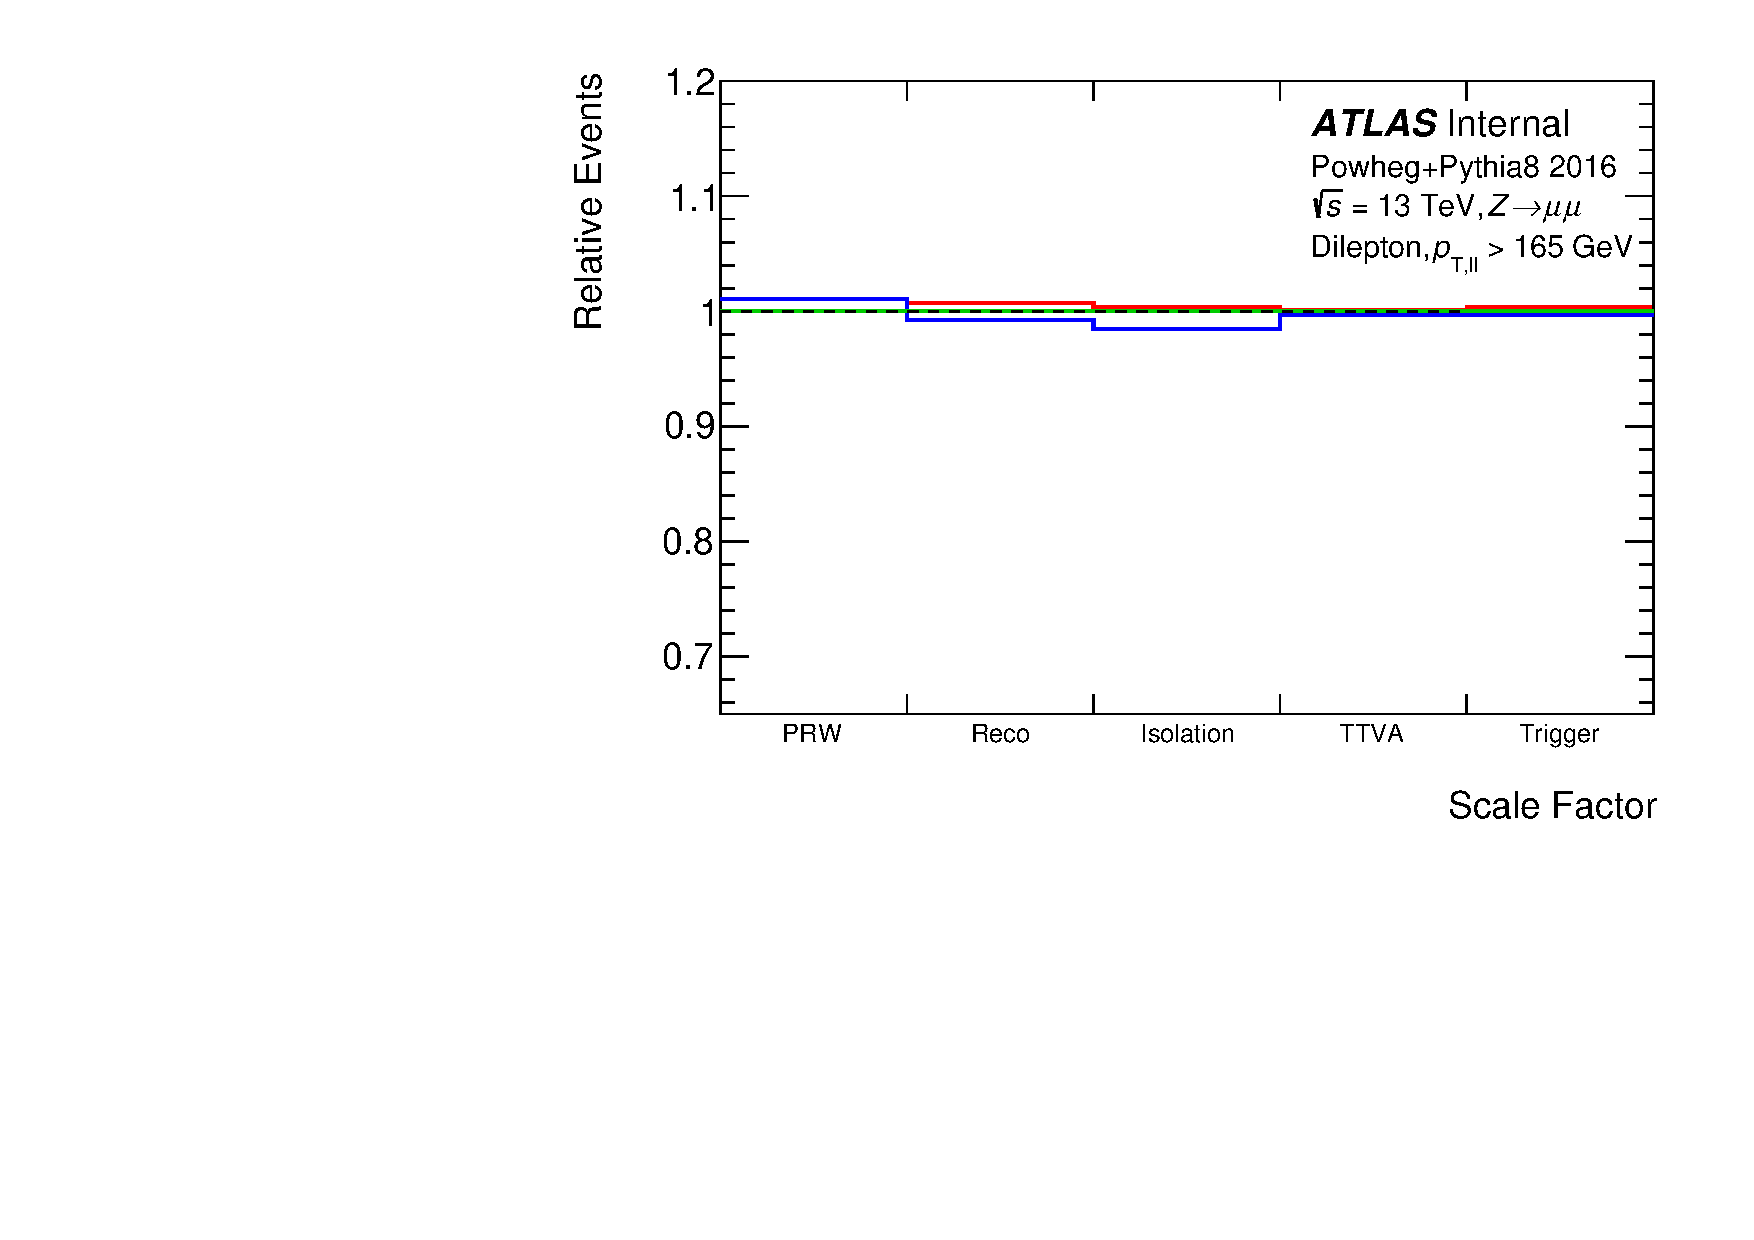
\includegraphics[page=1,width=0.45\textwidth]{figures/ZjetOmnifoldSystematics.pdf}}
  \subfloat[MC16d]{\includegraphics[page=103,width=0.45\textwidth]{figures/ZjetOmnifoldSystematics.pdf}} \\
  \subfloat[MC16e]{\includegraphics[page=205,width=0.45\textwidth]{figures/ZjetOmnifoldSystematics.pdf}}
  \subfloat[Run 2]{\includegraphics[page=307,width=0.45\textwidth]{figures/ZjetOmnifoldSystematics.pdf}}
  \caption{The fractional systematic impact of the up and down variations of the pileup reweighting across all years for the \powheg+\pythia~sample.}
  \label{fig:PRWpTll}
\end{figure}

\subsection{Muon uncertainties}
\label{sec:muonuncerts}

\subsubsection{Muon efficiency uncertainties}
As summarized in section~\ref{subsec:MCCorr} there are several scale factors associated with muon reconstruction related to efficiencies in the trigger, reconstruction, isolation and track-to-vertex association.
Hence, there are 2 systematic variations associated with the trigger efficiency, 2 for the isolation efficiency, 4 for the reconstruction efficiency, and 2 for the TTVA efficiency:
\begin{itemize}
  \setlength{\itemsep}{1pt}\setlength{\parskip}{0pt}\setlength{\parsep}{0pt}
  \item MUON\_EFF\_TrigSystUncertainty
  \item MUON\_EFF\_TrigStatUncertainty
  \item MUON\_EFF\_ISO\_SYS
  \item MUON\_EFF\_ISO\_STAT
  \item MUON\_EFF\_RECO\_SYS
  \item MUON\_EFF\_RECO\_SYS\_LOWPT
  \item MUON\_EFF\_RECO\_STAT
  \item MUON\_EFF\_RECO\_STAT\_LOWPT
  \item MUON\_EFF\_TTVA\_SYS
  \item MUON\_EFF\_TTVA\_STAT
\end{itemize}

The impact of the efficiency systematics is summarized in figure~\ref{fig:PP8SFSyst}.

\begin{figure}[h!]
  \centering
  \subfloat[MC16a]{\includegraphics[page=2,width=0.45\textwidth]{figures/ZjetOmnifoldSystematics.pdf}}
  \subfloat[MC16d]{\includegraphics[page=104,width=0.45\textwidth]{figures/ZjetOmnifoldSystematics.pdf}} \\
  \subfloat[MC16e]{\includegraphics[page=206,width=0.45\textwidth]{figures/ZjetOmnifoldSystematics.pdf}}
  \subfloat[Run 2]{\includegraphics[page=308,width=0.45\textwidth]{figures/ZjetOmnifoldSystematics.pdf}}
  \caption{The fractional systematic impact for the muon efficiencies for the \powheg+\pythia~samples across all years as a function of the dilepton \pt.}
  \label{fig:PP8SFSyst}
\end{figure}

\subsubsection{Muon calibration uncertainties}
There are also systematic variations associated with the calibration applied to the muons. These will have an affect on the muon kinematics. The systematic variations are listed below, and include
one for momentum variations due to measurements made in the inner detector, one for momentum effects related to the muon spectrometer, one for the momentum scale, and 2 systematics related to the measured sagitta value.
\begin{itemize}
  \setlength{\itemsep}{1pt}\setlength{\parskip}{0pt}\setlength{\parsep}{0pt}
  \item MUON\_ID (inner detector track resolution)
  \item MUON\_MS (muon spectrometer track resolution)
  \item MUON\_SCALE (momentum scale)
  \item MUON\_SAGITTA\_RESBIAS (residual bias correction)
  \item MUON\_SAGITTA\_RHO (combined measurement correction)
\end{itemize}

The effects of these variations on the dilepton \pt and mass are shown in figure~\ref{fig:PP8MuCalSystpTll} and~\ref{fig:PP8MuCalSystmll}.

\begin{figure}[h!]
  \centering
  \subfloat[MC16a]{\includegraphics[page=97,width=\textwidth]{figures/ZjetOmnifoldSystematics.pdf}} \\
  \subfloat[MC16d]{\includegraphics[page=199,width=\textwidth]{figures/ZjetOmnifoldSystematics.pdf}} \\
  \subfloat[MC16e]{\includegraphics[page=301,width=\textwidth]{figures/ZjetOmnifoldSystematics.pdf}} \\
  \subfloat[Run 2]{\includegraphics[page=403,width=\textwidth]{figures/ZjetOmnifoldSystematics.pdf}}
  \caption{The fractional systematic impact for variations to the muon calibration for the \powheg+\pythia~samples for all years as a function of the dilepton \pt. The upwards shift is presented in red, and the downwards shift in blue.}
  \label{fig:PP8MuCalSystpTll}
\end{figure}

\begin{figure}[h!]
  \centering
  \subfloat[MC16a]{\includegraphics[page=99,width=\textwidth]{figures/ZjetOmnifoldSystematics.pdf}} \\
  \subfloat[MC16d]{\includegraphics[page=201,width=\textwidth]{figures/ZjetOmnifoldSystematics.pdf}} \\
  \subfloat[MC16e]{\includegraphics[page=303,width=\textwidth]{figures/ZjetOmnifoldSystematics.pdf}} \\
  \subfloat[Run 2]{\includegraphics[page=405,width=\textwidth]{figures/ZjetOmnifoldSystematics.pdf}}
  \caption{The fractional systematic impact for variations to the muon calibration for the \powheg+\pythia~samples for all years as a function of the dilepton mass. The upwards shift is presented in red, and the downwards shift in blue.}
  \label{fig:PP8MuCalSystmll}
\end{figure}

\subsection{Track uncertainties}

The systematic uncertainties associated with the tracks are:

\begin{itemize}
  \setlength{\itemsep}{1pt}\setlength{\parskip}{0pt}\setlength{\parsep}{0pt}
  \item InDet::TRK\_EFF\_TIGHT\_GLOBAL
  \item InDet::TRK\_EFF\_TIGHT\_IBL
  \item InDet::TRK\_EFF\_TIGHT\_PP0
  \item InDet::TRK\_EFF\_TIGHT\_PHYSMODEL
  \item InDet::TRK\_EFF\_LOOSE\_TIDE
  \item InDet::TRK\_FAKE\_RATE\_LOOSE
  \item InDet::TRK\_BIAS\_QOVERP\_SAGITTA\_WM
\end{itemize}

The first four are combined into one nuisance parameter and are due to variations of the tracking efficiency. The fifth describes the variations to the tracking efficiency when the track is inside a jet.
The sixth represents variations to the fake rate. The last varies the \pt of the track based on the residual alignment uncertainties. Figure~\ref{fig:PP8TrackSyst} shows the effect of these variations on the \pt of the tracks in the \powheg+\pythia~sample across all years.

\begin{figure}[h!]
  \centering
  \subfloat[MC16a]{\includegraphics[page=102,width=0.45\textwidth]{figures/ZjetOmnifoldSystematics.pdf}}
  \subfloat[MC16d]{\includegraphics[page=204,width=0.45\textwidth]{figures/ZjetOmnifoldSystematics.pdf}} \\
  \subfloat[MC16e]{\includegraphics[page=306,width=0.45\textwidth]{figures/ZjetOmnifoldSystematics.pdf}}
  \subfloat[Run 2]{\includegraphics[page=408,width=0.45\textwidth]{figures/ZjetOmnifoldSystematics.pdf}}
  \caption{The fractional systematic impact for variations applied to the tracks for the \powheg+\pythia~samples for all years. Note that only the down variations are shown for the inclusive efficiency, inside jet efficiency and the fake rate.
  The variations are symmetrized for use in the analysis.}
  \label{fig:PP8TrackSyst}
\end{figure}

The track systematics will also have an effect on the track jet observables. Figure~\ref{fig:PP8TrackJetSyst} shows the fractional effect of the track systematics on the \pt, $y$, $m$, $\tau_1$, and the number of constituents of the leading track jet.

\begin{figure}[h!]
  \centering
  \subfloat{\includegraphics[page=332,width=0.45\textwidth]{figures/ZjetOmnifoldSystematics.pdf}}
  \subfloat{\includegraphics[page=335,width=0.45\textwidth]{figures/ZjetOmnifoldSystematics.pdf}} \\
  \subfloat{\includegraphics[page=341,width=0.45\textwidth]{figures/ZjetOmnifoldSystematics.pdf}}
  \subfloat{\includegraphics[page=344,width=0.45\textwidth]{figures/ZjetOmnifoldSystematics.pdf}} \\
  \subfloat{\includegraphics[page=374,width=0.45\textwidth]{figures/ZjetOmnifoldSystematics.pdf}}
  \caption{The fractional systematic impact of the track variations on various track jet observables for the full Run 2 dataset of the \powheg+\pythia~sample.}
  \label{fig:PP8TrackJetSyst}
\end{figure}

\subsection{Modeling and unfolding uncertainties}

Modeling uncertainties are determined by unfolding the data with simulations that have different physics models.  We will do this by first comparing the result when unfolding with \pythia{} and when unfolding with \sherpa.  This is a crude uncertainty because there are multiple differences between these generators.  We will complement this comparison by unfolding with various \powheg+\pythia{} samples (see Sec.~\ref{sec:theoryuncerts}) that have been re-weighted based on truth-level samples that have targeted variations (e.g.\ A14 tune variations).  Additional samples are being prepared by the PMG but will likely not be ready in time for this analysis.

Unfolding uncertainties are designed to quantify the method closure.  We will do this by unfolding \pythia{} with \sherpa{} and then comparing to the \pythia{} truth (and vice versa).  This may have some double-counting with modeling uncertainties and is often mitigated by performing some reweighting\footnote{\url{https://twiki.cern.ch/twiki/bin/viewauth/AtlasProtected/StandardModelUnfolding}}~\cite{Malaescu:2009dm} (which actually is similar to OmniFold Step 1).  However, we will choose the more conservative approach for this first high-dimensional analysis.

\clearpage

\subsection{Theoretical uncertainties}
\label{sec:theoryuncerts}
\subsubsection{QCD renormalization and factorization scale variations}
The variation of the QCD renormalization ($\mu_r$) and factorization ($\mu_f$) scale on the process was studied using the \sherpa\ event generator (one of our nominal samples).
This sample contains event weights corresponding to the standard variations of $\times 2$ and $\times 0.5$ for each scale.
%This generator can vary each scale independently and provides combinations of up (2$\mu_(r,f)$) and down (0.5$\mu_(r,f)$) variations of each scale.
The impact of each variation relative to the nominal scale choice is shown in figure~\ref{fig:QCDscale_mjj}.
Both $\mu_r$ and $\mu_f$ varied up is denoted ``uu'' and both varied down ``dd'', while ``n" indicates the nominal quantity etc.
A larger renormalization scales results in a smaller cross section and hence less events in the observed dilepton \pt spectrum, and vice versa.
Varying the factorization scale has very little impact.

\begin{figure}[h!]
  \centering
  \subfloat[MC16a]{\includegraphics[page=2,width=0.45\textwidth]{figures/systQCD.pdf}}
  \subfloat[MC16d]{\includegraphics[page=4,width=0.45\textwidth]{figures/systQCD.pdf}} \\
  \subfloat[MC16e]{\includegraphics[page=6,width=0.45\textwidth]{figures/systQCD.pdf}}
  \subfloat[Run 2]{\includegraphics[page=7,width=0.45\textwidth]{figures/systQCD.pdf}}
  \caption{The fractional impact of the QCD scale variations for the \sherpa~samples on the dilepton \pt spectrum for all the years and full Run2. The result of varying $\mu_r$ and $\mu_f$ in the up direction is shown in dark red and the downwards shift is in dark blue color. The lighter blue and red show the result of only varying $\mu_r$, and the green lines only varying $\mu_f$.}
  \label{fig:QCDscale_mjj}
\end{figure}

\subsubsection{Parton Shower (PS) uncertainties}
To compute the parton shower uncertainties, \powheg$+$\pythia~samples with the AZNLO tune are used (listed in appendix~\ref{app:datasets}). These samples are customized using a standard dilepton \pt filter ($\pt^{\ell\ell}\geq100$ GeV), the detailed JOs and preliminarily validation plots can be found at the JIRA ticket for the sample request~\url{https://its.cern.ch/jira/browse/ATLMCPROD-9320}. A set of systematic variations is provided for the AZNLO tune, based on the eigentune method. In order to cover the full range of PS uncertainties, a subset of tune variations which together provide maximal coverage of the observables: one pair mainly for underlying event effects (Var1), one pair mainly for jet structure effects (Var2), along with scale variations (RenUp and RenDown) and MultipartonInteractions (MPI) variations (MPIUp and MPIDown) is used. The impact of these variation relative to the nominal sample is shown in figure~\ref{fig:PS_MPI}.

\begin{figure}[h!]
  \centering
  \subfloat[]{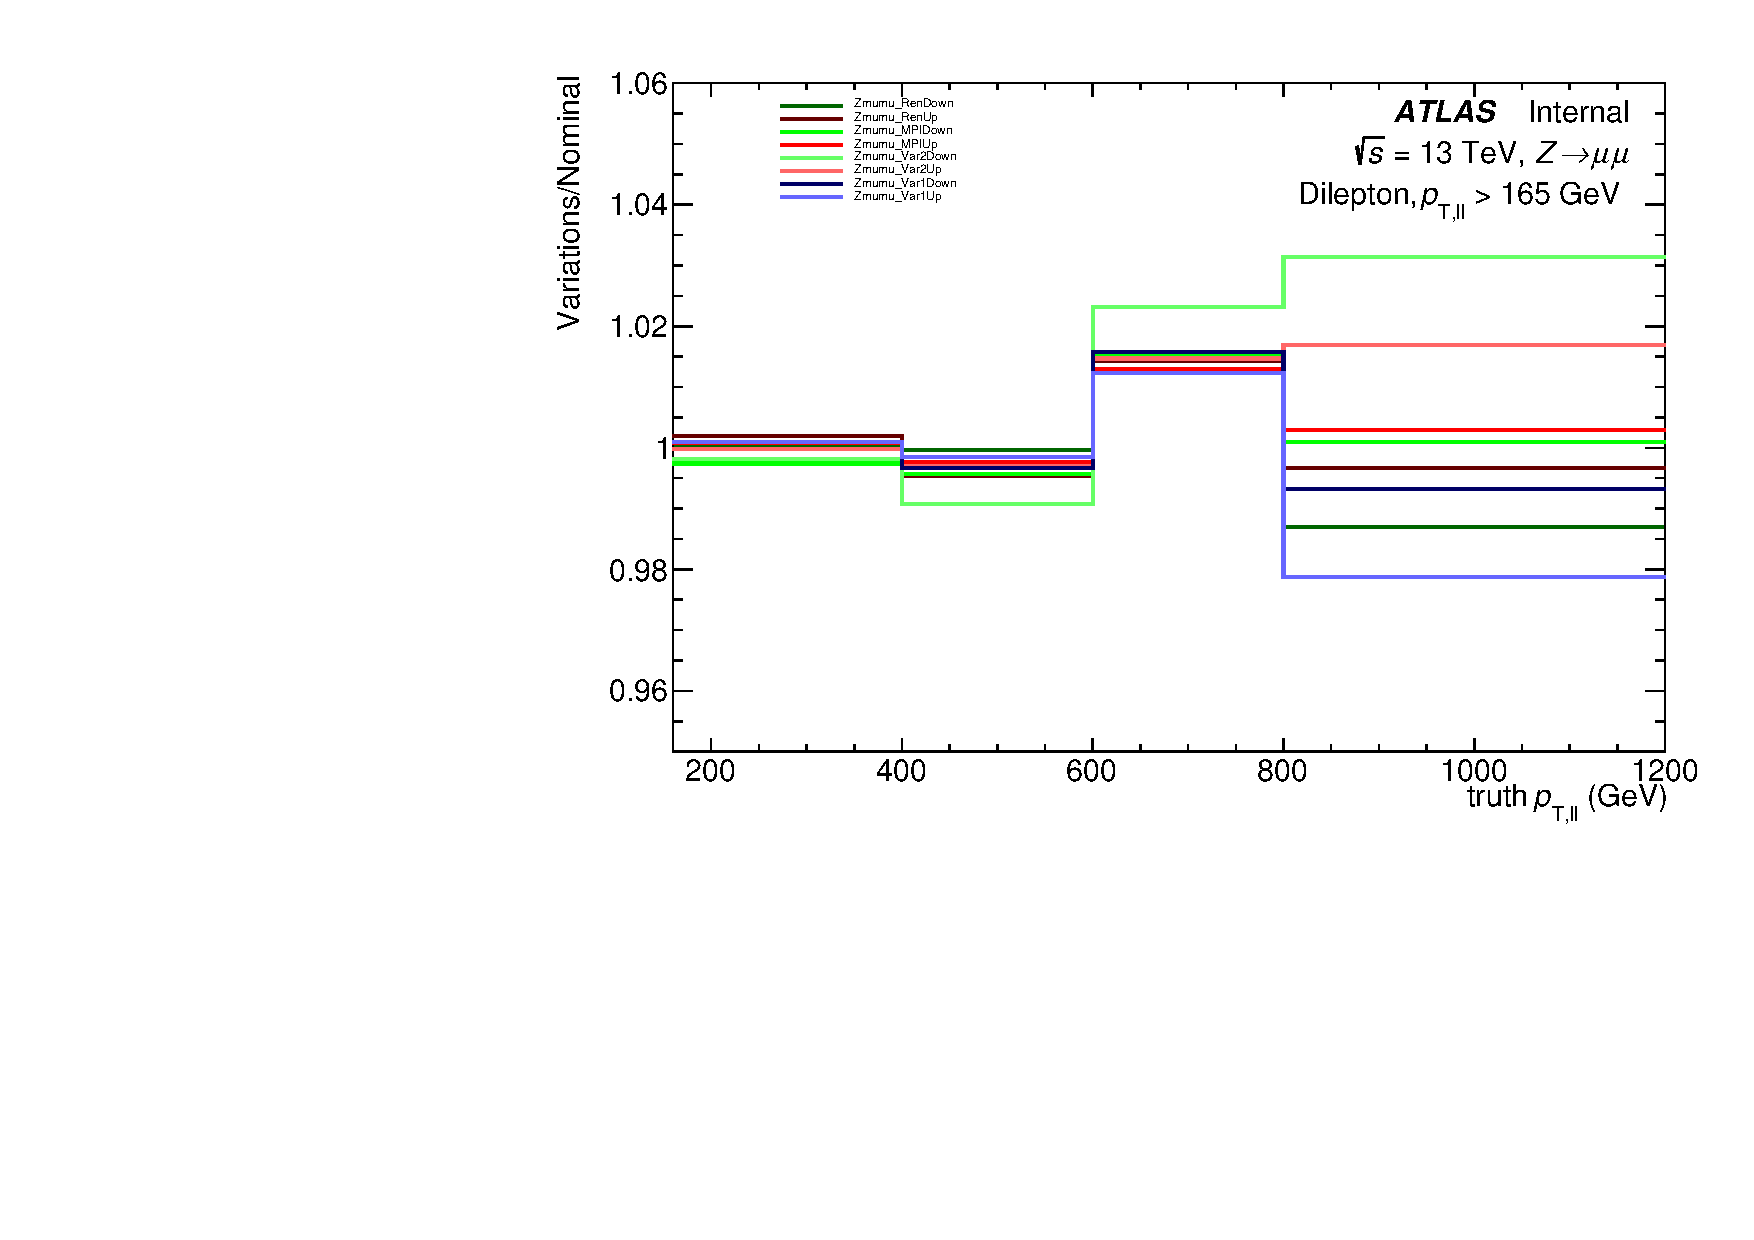
\includegraphics[page=1,width=0.45\textwidth]{figures/ShowerVartions_pTll.pdf}}
  \subfloat[]{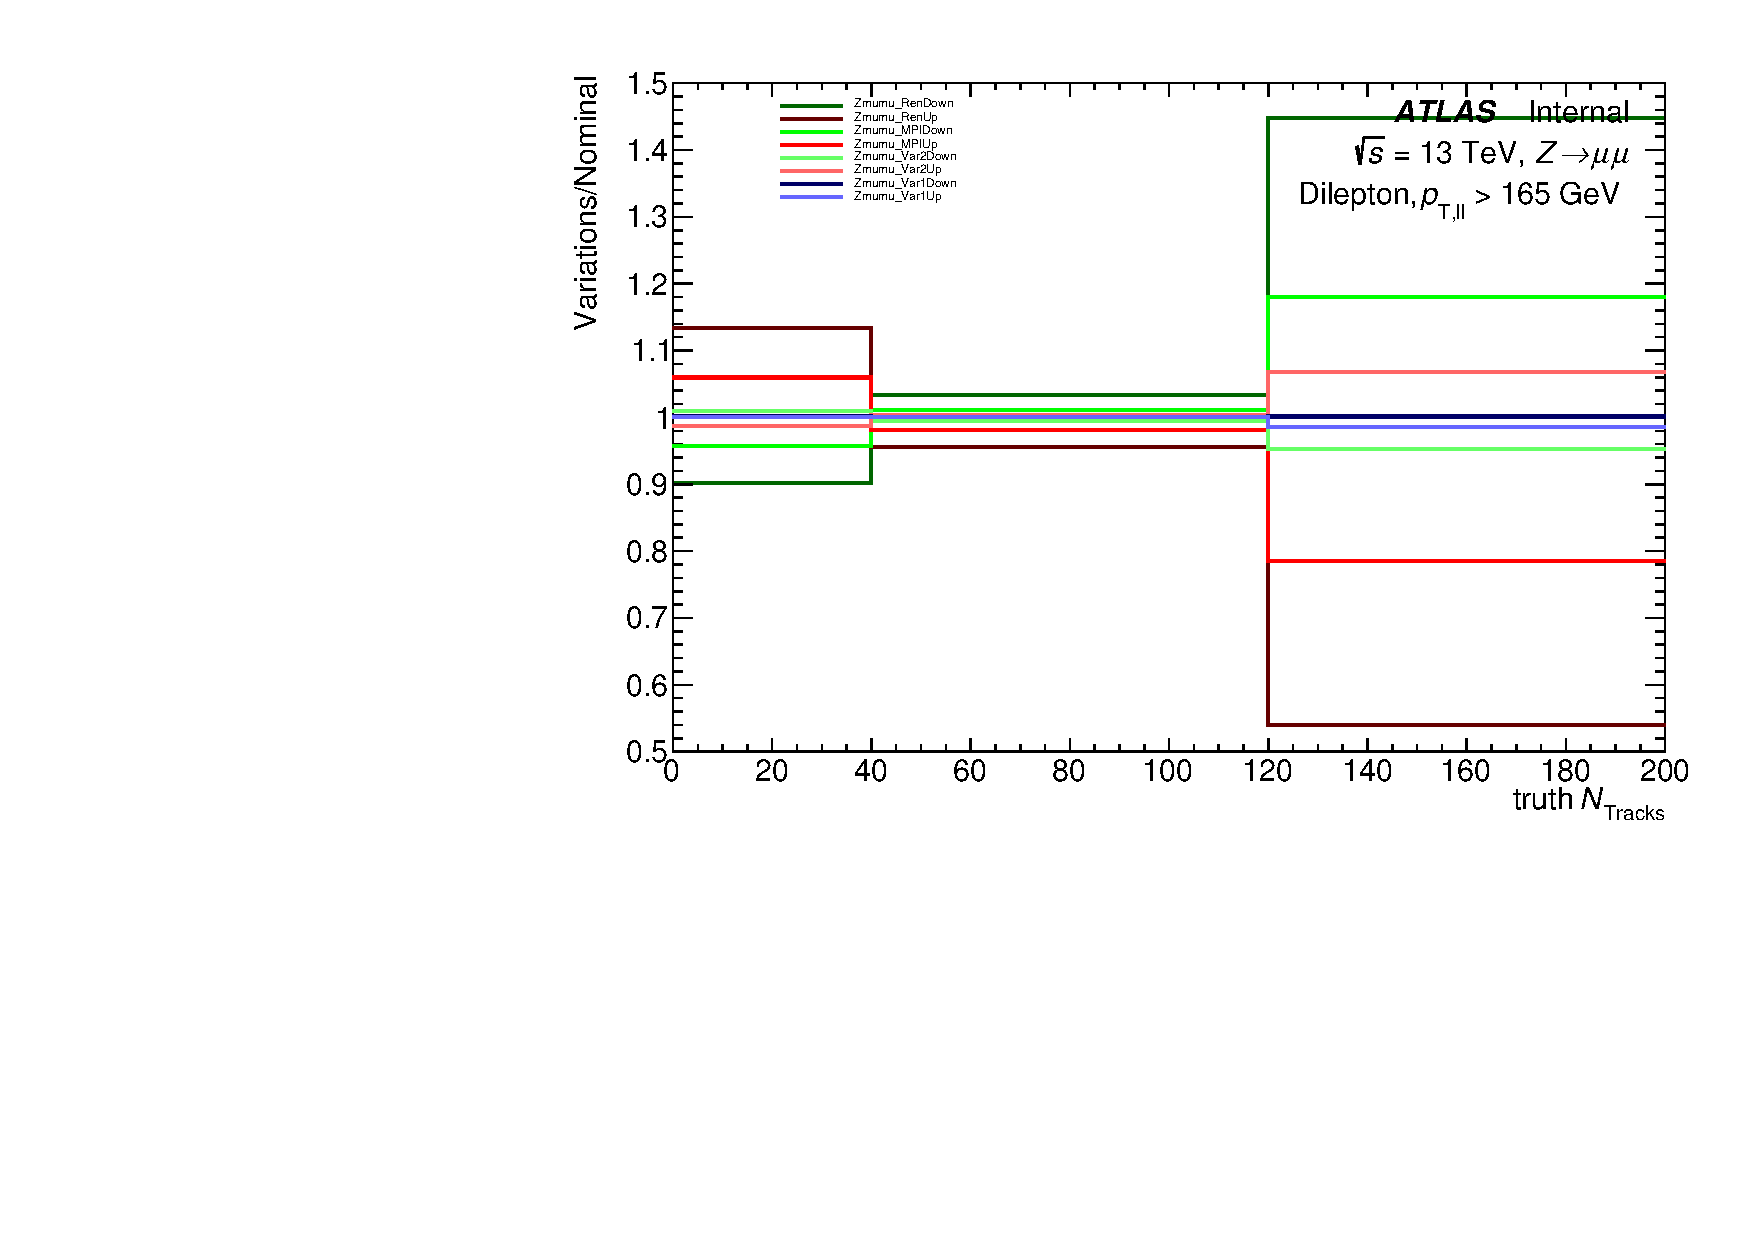
\includegraphics[page=1,width=0.45\textwidth]{figures/ShowerVartions_Ntracks.pdf}} \\
  \subfloat[]{\includegraphics[page=2,width=0.45\textwidth]{figures/ShowerVartions_Ntracks.pdf}}
  \subfloat[]{\includegraphics[page=3,width=0.45\textwidth]{figures/ShowerVartions_Ntracks.pdf}}\\
  \subfloat[]{\includegraphics[page=4,width=0.45\textwidth]{figures/ShowerVartions_Ntracks.pdf}}
  \subfloat[]{\includegraphics[page=2,width=0.45\textwidth]{figures/ShowerVartions_etaTracks.pdf}}
  \caption{The fractional impact of the MC tuning and MPI variations for the \pythia~samples on the track jet properties and dilepton \pt for full Run2. Systematic effect evaluated by varying different parameters of the MC samples. The statistical uncertainties on these uncertainties are about 0.001\%, 0.05\% and 3\% in the three bins.}
  \label{fig:PS_MPI}
\end{figure}

\subsubsection{Parton Distribution Function (PDF) variations}
The variability of the underlying PDF is calculated using the \sherpa~samples (listed in appendix~\ref{app:datasets}). The nominal PDF used by the generator is the central value of some underlying PDF distribution, the \sherpa~generator provides 100 variations to this nominal pdf that are generated from this underlying statistical distribution.  The RMS of these 100 results is interpreted as a systematic uncertainty, this spread is shown for the measurement in figure~\ref{fig:PDF_RMS}. Also the fractional impact of the $\alpha_{s}$ variations and two alternative PDF sets is shown in figure~\ref{fig:alpha_S}.
\begin{figure}[h!]
  \centering
  \subfloat[]{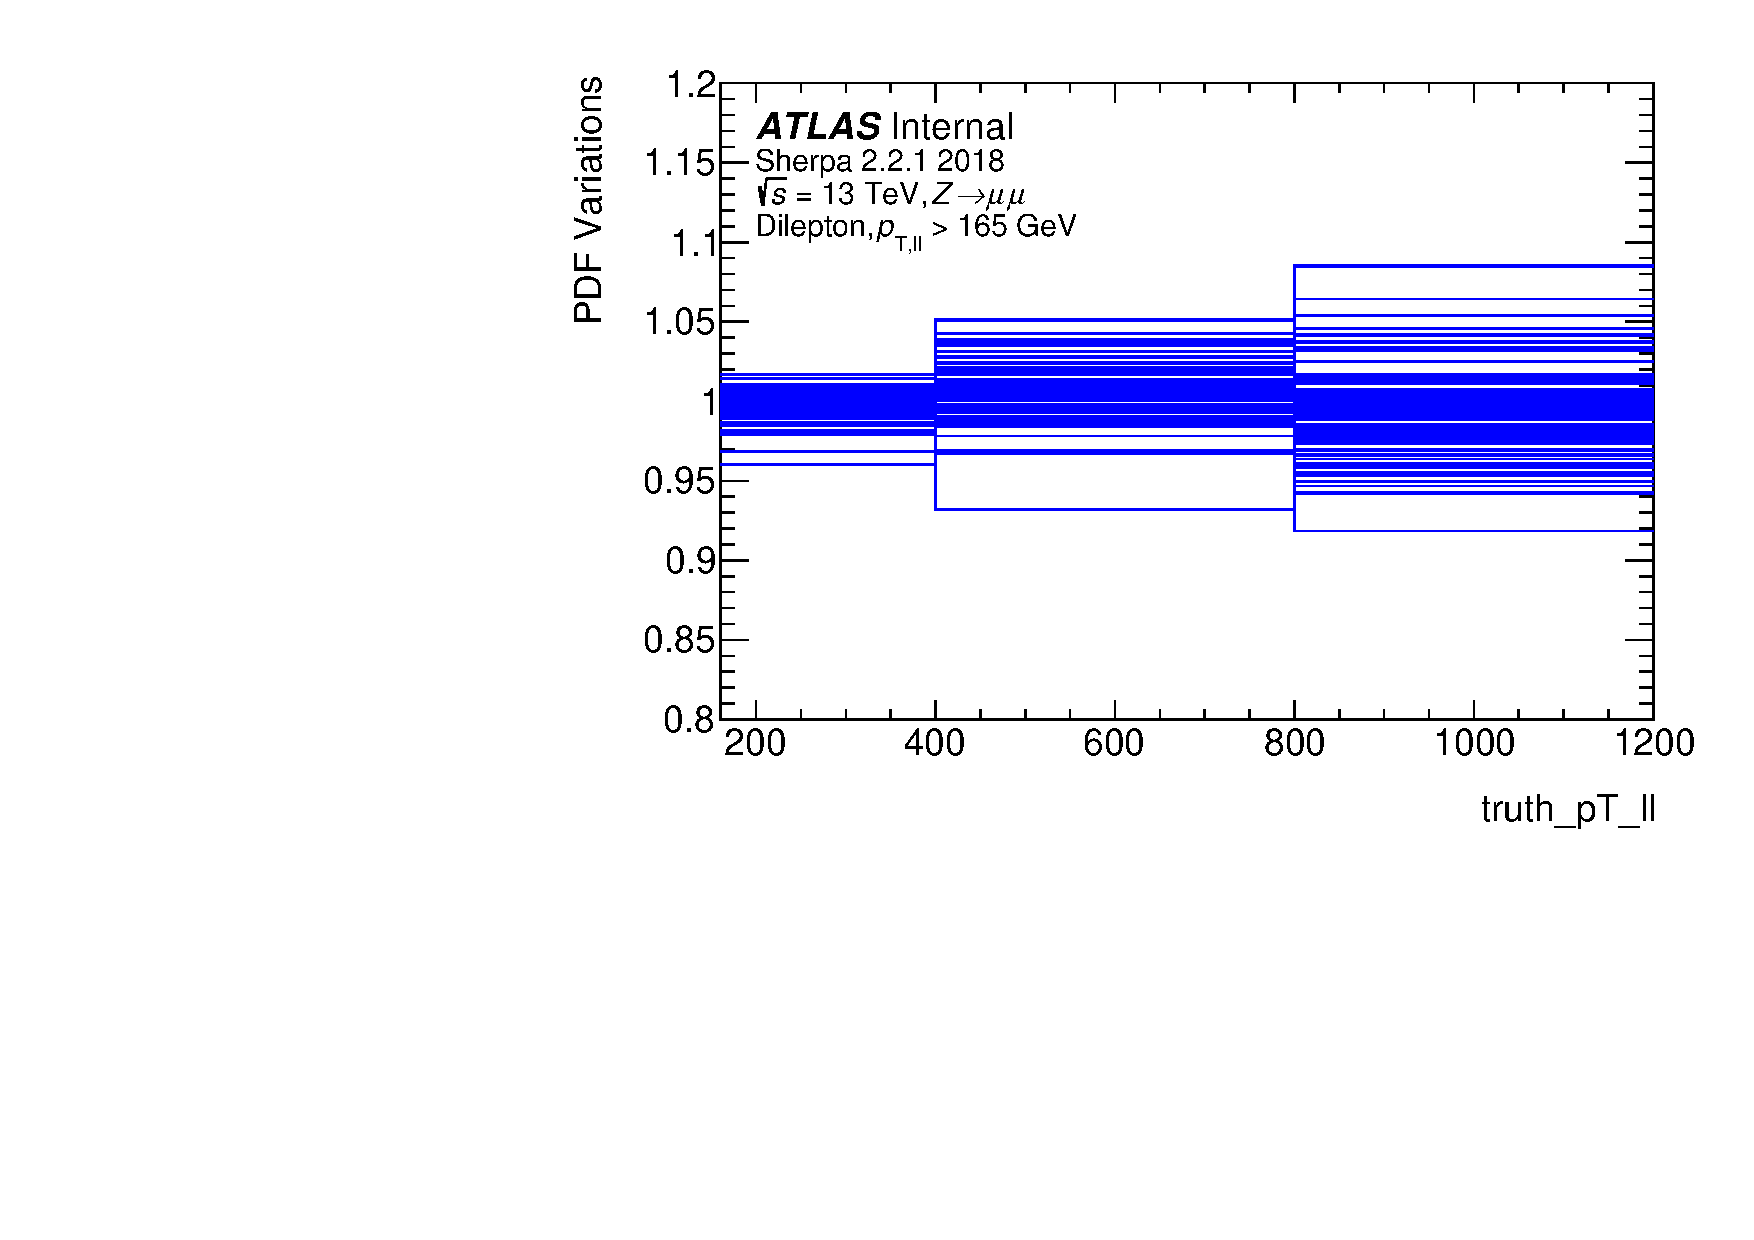
\includegraphics[page=1,width=0.45\textwidth]{figures/systPDF_100.pdf}}
  \subfloat[]{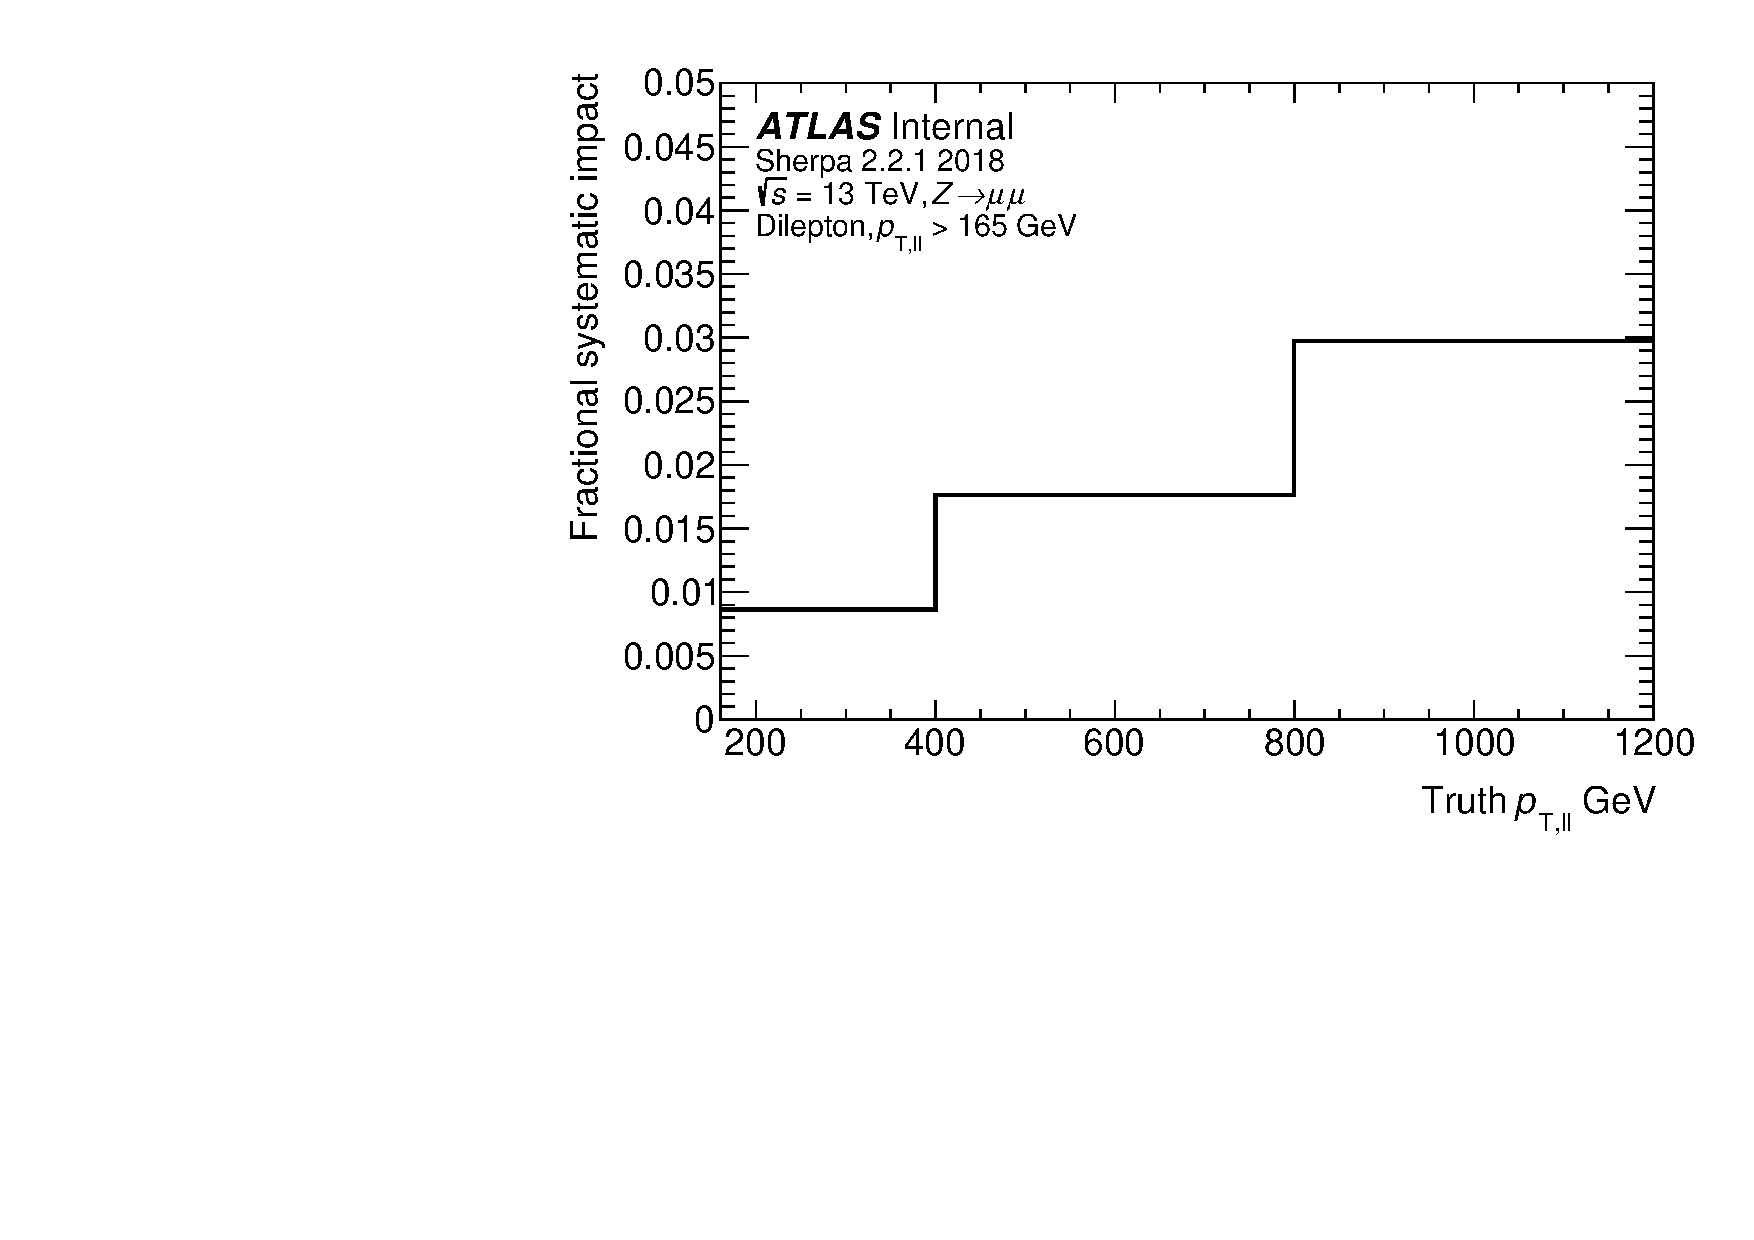
\includegraphics[page=1,width=0.45\textwidth]{figures/systPDF_RMS.pdf}} \\
  \caption{Spread of 100 PDF variations per bin (left) and impact of systematic uncertainty as RMS of these 100 results (right) on dilepton \pt. To show smooth variations in these plots, some events with large negative weights are skipped.}
  \label{fig:PDF_RMS}
\end{figure}

\begin{figure}[h!]
  \centering
  \includegraphics[page=2,width=0.45\textwidth]{figures/syst_alphaS.pdf} \\
  \caption{The fractional impact of the $\alpha_{s}$ variations for the \sherpa~samples on the dilepton \pt spectrum. The result of varying $\alpha_{s}$ in the up direction is shown in dark red and the downwards shift is in dark blue color. The lighter green and black color show uncertainty for the two alternative PDF sets.}
  \label{fig:alpha_S}
\end{figure}
